\begin{figure}
\usetikzlibrary{patterns}
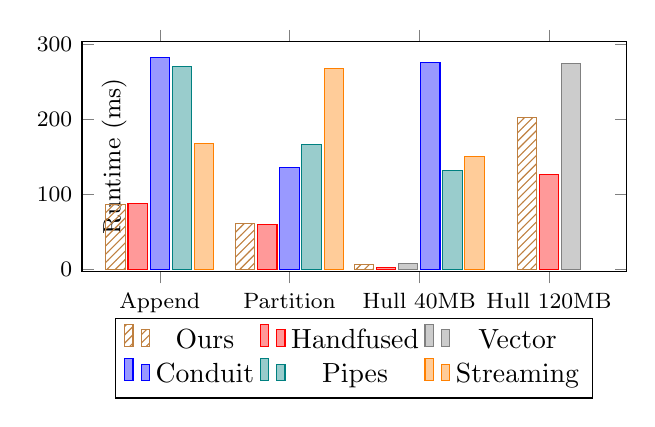
\begin{tikzpicture}

% Bar chart for benchmarks:
% This is a complicated bar chart because there are six series (conduit, pipes, vector..), but they are not all defined at all points (append, partition, quickhull).
% We need to split it into three different pictures, overlaid on top of each other.
% The first picture just defines the legend, the axis labels, etc.
\begin{axis}[
  symbolic x coords={Append, Partition, Hull 40MB, Hull 120MB, end},
  xtick=data, ylabel=Runtime (ms),
y label style={at={(axis description cs:0.1,.5)},anchor=south},
  % All pictures need to specify same upper and lower bounds so they line up together
  ymin=0, ymax=300,
  xmin=Append, xmax=Hull 120MB,
        enlargelimits=0.01,
  enlarge x limits=0.20,
        ybar=1pt,
        bar width=7pt,
        small,
  width=8.5cm, height=4.5cm,
  legend style={at={(0.5,-0.2)},anchor=north, legend columns=3},
]
% The colours need to be specified manually, to force the legend entries to show up..
% The colours also need to match the colours specified for each series data.
\addlegendimage{brown,pattern=north east lines,pattern color=brown}
\addlegendimage{red,fill=red!40!white}
\addlegendimage{gray,fill=gray!40!white}
\addlegendimage{blue,fill=blue!40!white}
\addlegendimage{teal,fill=teal!40!white}
\addlegendimage{orange,fill=orange!40!white}
\legend{Ours, Handfused, Vector, Conduit, Pipes, Streaming}
\addplot[white] coordinates {(Append,  0) (Partition,  0)  (Hull 40MB, 0) (Hull 120MB, 0)  };
\end{axis}

\begin{axis}[
  symbolic x coords={Append, Partition, Hull 40MB, Hull 120MB, end},
  ticks=none,
  ymin=0, ymax=300,
  xmin=Append, xmax=Hull 120MB,
        enlargelimits=0.01,
  enlarge x limits=0.20,
        ybar=1pt,
        bar width=7pt,
        small,
  width=8.5cm, height=4.5cm,
  legend style={at={(0.5,-0.2)},anchor=north, legend columns=3},
]
% Ours
\addplot[brown,pattern=north east lines,pattern color=brown] coordinates {(Append,  86) (Partition,  61)   };
% Handfused
\addplot[red,fill=red!40!white] coordinates {(Append,  88) (Partition,  60)   };
% Conduit
\addplot[blue,fill=blue!40!white] coordinates {(Append, 282) (Partition, 136)   };
% Pipes
\addplot[teal,fill=teal!40!white] coordinates {(Append, 270) (Partition, 166)  };
% Streaming
\addplot[orange,fill=orange!40!white] coordinates {(Append, 168) (Partition, 268)  };
\end{axis}

\begin{axis}[
  symbolic x coords={Append, Partition, Hull 40MB, Hull 120MB, end},
  ticks=none,
  ymin=0, ymax=300,
  xmin=Append, xmax=Hull 120MB,
        enlargelimits=0.01,
  enlarge x limits=0.20,
        ybar=1pt,
        bar width=7pt,
        small,
  width=8.5cm, height=4.5cm,
  legend style={at={(0.5,-0.2)},anchor=north, legend columns=3},
]
% Ours
\addplot[brown,pattern=north east lines,pattern color=brown] coordinates {(Hull 40MB, 6) };
% Handfused
\addplot[red,fill=red!40!white] coordinates {(Hull 40MB,  3) };
% Vector
\addplot[gray,fill=gray!40!white] coordinates {(Hull 40MB, 8)  };
% Conduit
\addplot[blue,fill=blue!40!white] coordinates {(Hull 40MB, 275)  };
% Pipes
\addplot[teal,fill=teal!40!white] coordinates {(Hull 40MB, 132) };
% Streaming
\addplot[orange,fill=orange!40!white] coordinates {(Hull 40MB, 150) };
\end{axis}

\begin{axis}[
  symbolic x coords={Append, Partition, Hull 40MB, Hull 120MB, end},
  ticks=none,
  ymin=0, ymax=300,
  xmin=Append, xmax=Hull 120MB,
        enlargelimits=0.01,
  enlarge x limits=0.20,
        ybar=1pt,
        bar width=7pt,
        small,
  width=8.5cm, height=4.5cm,
  legend style={at={(0.5,-0.2)},anchor=north, legend columns=3},
]
% Ours
\addplot[brown,pattern=north east lines,pattern color=brown] coordinates {  (Hull 120MB, 202)  };
% Handfused
\addplot[red,fill=red!40!white] coordinates {  (Hull 120MB, 126)  };
% Vector
\addplot[gray,fill=gray!40!white] coordinates {(Hull 120MB, 274)  };
\end{axis}

\end{tikzpicture}
\caption{Runtime for benchmarks; lower is faster.}
\label{fig:bench:all}
\end{figure}


